\documentclass[tikz]{standalone}

\begin{document}

\bfseries 
\footnotesize 
\begin{tikzpicture}[line width=0.8mm,scale=1.4]

	% === REFFERENCES === (((
	\node [opacity=0.7] at (0,0) 
	{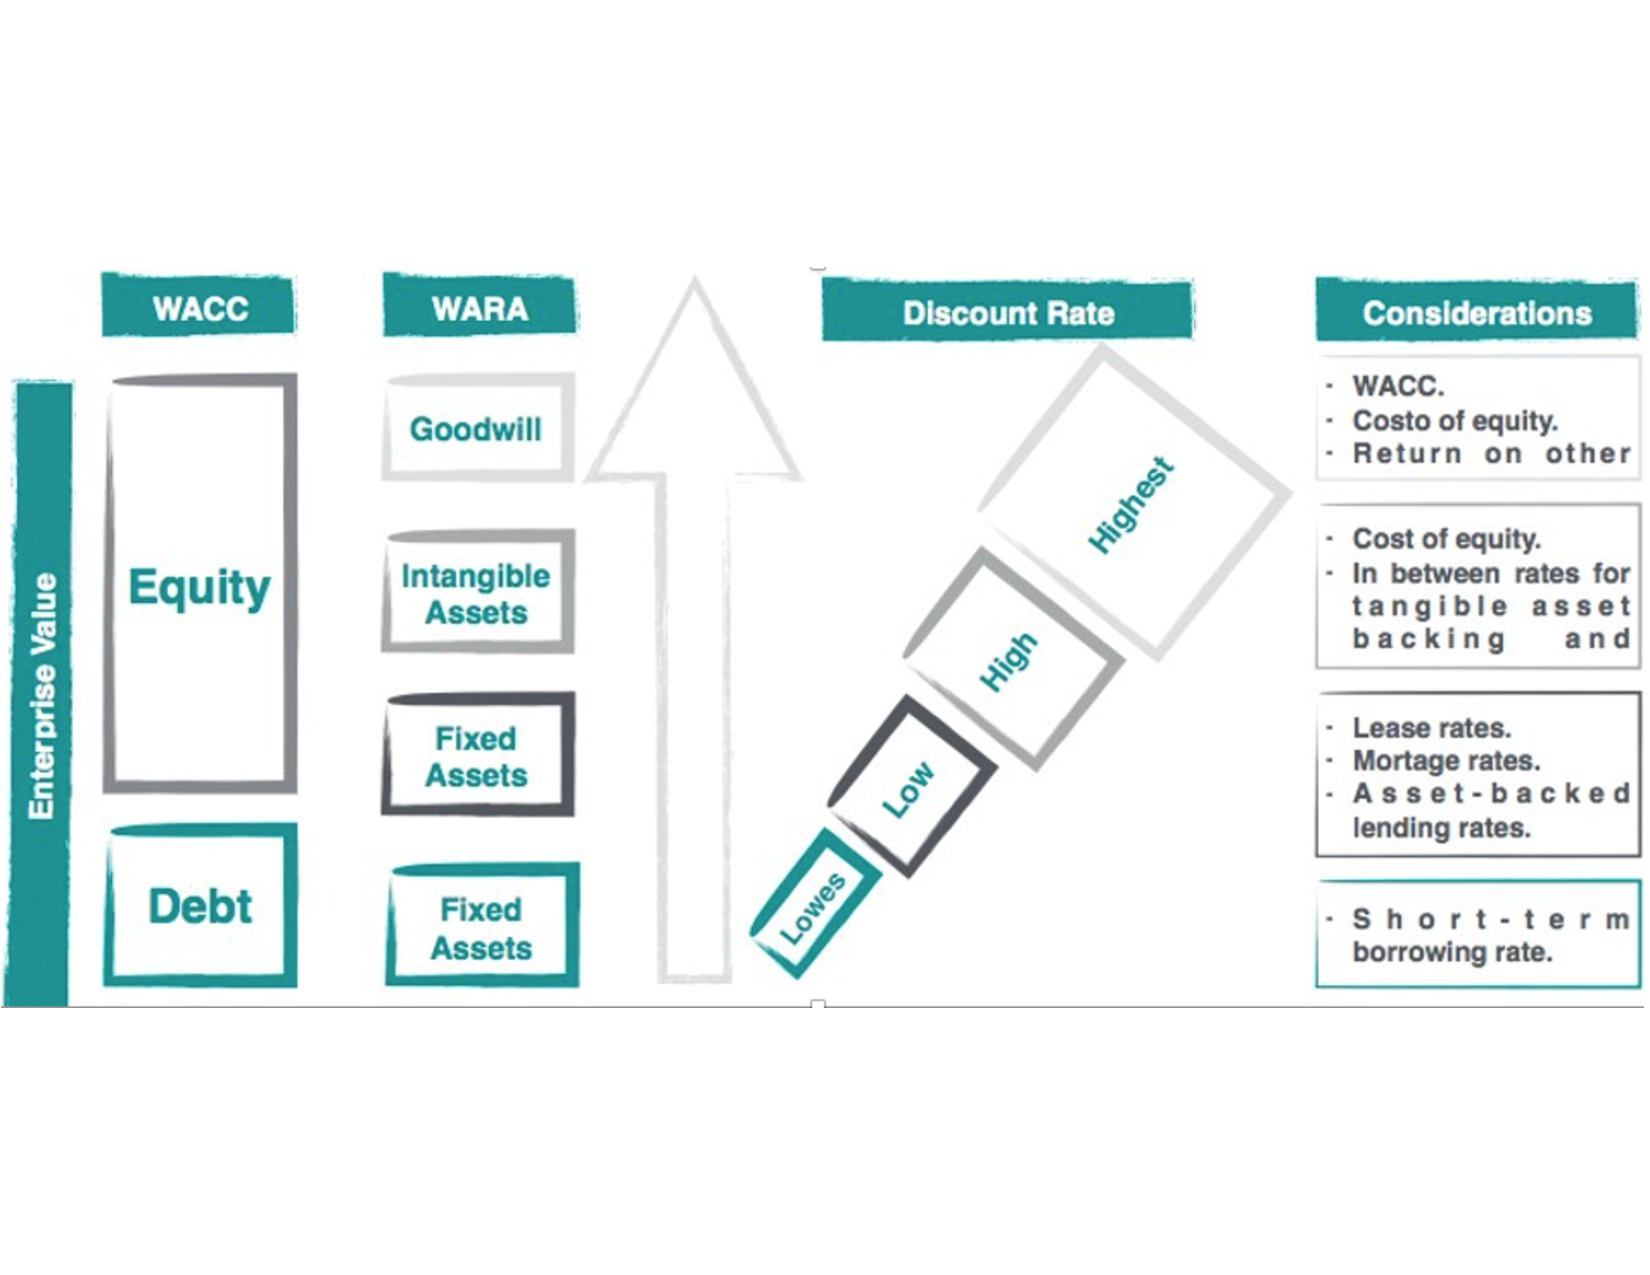
\includegraphics[width=  14cm, page = 1]{image}};
	\draw [help lines] (-5,-2.5) grid (5,2.5);
	\fill [red] (0,0) circle (2pt);
	% )))

	\draw [gray] (-4.4,-0.9) rectangle node [text=teal] 
	{\large Capital} ++(1.3,2.5);
	\fill [teal] (-4.9,-2.3) rectangle 
	node [rotate=90,text=white] {Valor Emmpresarial} ++(0.3,4);
	\draw [teal] (-4.4,-2.1) rectangle node {Deuda} ++(1.3,1);
	\fill [teal] (-4.4,1.85) rectangle 
	node [text=white] {WACC} ++(1.3,0.3);
	\fill [teal] (-2.7,1.85) rectangle 
	node [text=white] {WARA} ++(1.3,0.3);
	\draw [gray!40] (-2.7,0.95) rectangle 
	node [text=teal] {Goodwill} ++(1.15,0.7);
	\draw [gray!80] (-2.7,-0.05) rectangle 
	node [text=teal] {\shortstack{Intangible \\ Assets}} ++(1.15,0.7);
	\draw [gray] (-2.7,-1.1) rectangle 
	node [text=teal] {\shortstack{Fixed \\ Assets}} ++(1.15,0.7);
	\draw [teal] (-2.7,-2.1) rectangle 
	node {\shortstack{Fixed \\ Assets}} ++(1.15,0.7);
	% \draw [gray!40] 
	% (-1,-2.1) -- ++(0.45,0) --++ (0,4.1) --++ (0.45,0) 
	% --++ () <++>
	% ;


\end{tikzpicture}

\end{document}
